\documentclass[12pt]{article}

\title{Everloyal}
\author{John Conway}

%PACKAGES
\usepackage[utf8]{inputenc}    
\usepackage[T1]{fontenc}
\usepackage[table]{xcolor}
\usepackage{ebgaramond}
\usepackage[left=0.75in, right=0.75in, top=0.75in, bottom=0.5in]{geometry}
\usepackage{tcolorbox}    
\usepackage{sectsty}
\usepackage{tikz}    
\usepackage{graphicx}
\usepackage{framed}
\usepackage{multicol}
\usepackage{pdfpages}
\usepackage[hidelinks]{hyperref}
\usepackage{titlesec}
\usepackage{lipsum}
\usepackage{tocloft}
\usepackage{pbox}
\usepackage{tabularx}
\usepackage{eso-pic,graphicx}
\usepackage{makecell}

%SETTINGS
\setlength{\columnsep}{2em}
\setcellgapes{12pt}

%COMMANDS
\newcommand{\makeref}[1]{\hypertarget{#1}{\textbf{#1}}}
\newcommand{\makerefit}[1]{\hypertarget{#1}{\emph{#1}}}
\newcommand{\makerefn}[1]{\hypertarget{#1}{#1}}

\newcommand{\refto}[1]{\hyperlink{#1}{\textbf{#1}}}
\newcommand{\reftoit}[1]{\hyperlink{#1}{\emph{#1}}}
\newcommand{\refton}[1]{\hyperlink{#1}{#1}}

\newcommand{\encountersection}[3]{
	\pagebreak
	\hypertarget{#1#2}{\subsection*{#1#2\hfill #3}\label{#1#2}}
	\input{chapsections/#1/#2}
	\pagebreak
}

\newcommand{\chapsection}[3]{
	{\hypertarget{#1#2}{}}
	\begin{tcolorbox}
	[colback=gray!5!white,colframe=gray!75!black,title=\subsection*{#1#2\hfill #3}\label{#1#2}]
	\input{chapsections/#1/#2}
	\end{tcolorbox}
}

\newcommand{\turnto}[1]{\hyperlink{#1}{\textbf{Turn to Page:} \pageref*{#1}:#1}}

\newcommand{\makefellow}[1]{\hypertarget{#1}{\subsection{#1}}}
\newcommand{\fellow}[1]{\hyperlink{#1}{> \textbf{Fellow:} #1}}

\newcommand{\requires}[1]{>> \emph{#1:}}
\newcommand{\requiresx}[1]{> \emph{#1:}}

\newcommand{\makeitem}[1]{#1\hypertarget{#1}{}\label{#1}}

\newcommand{\gain}[1]{> \textbf{Gain:} \hyperlink{#1}{#1 (Page: \pageref*{#1})}}
\newcommand{\gainx}[1]{>> \textbf{Gain:} \hyperlink{#1}{#1 (Page: \pageref*{#1})}}
\newcommand{\listitem}[1]{\hyperlink{#1}{#1 (Page: \pageref*{#1})}}

\newcommand{\notegain}[1]{>> \textbf{Mark #1} --}
\newcommand{\notegainx}[1]{\textbf{Mark #1} --}

\def\lisp{{\footnotesize \emph{th}}}
\def\lispx{{\footnotesize \emph{th }}}

\makeatletter
\@ifundefined{c@rownum}{%
  \let\c@rownum\rownum
}{}
\@ifundefined{therownum}{%
  \def\therownum{\@arabic\rownum}%
}{}
\makeatother

%COLUMNS
\newcolumntype{L}{>{\raggedright\arraybackslash}m{5cm}}
\newcolumntype{s}{>{\raggedright\arraybackslash}m{3cm}}
\newcolumntype{C}{>{\centering\arraybackslash}m{5cm}}

%DOCUMENT
\begin{document}
\hbadness=10001
\hfuzz=10001pt
\newpage 
\thispagestyle{empty}
\pagenumbering{gobble}
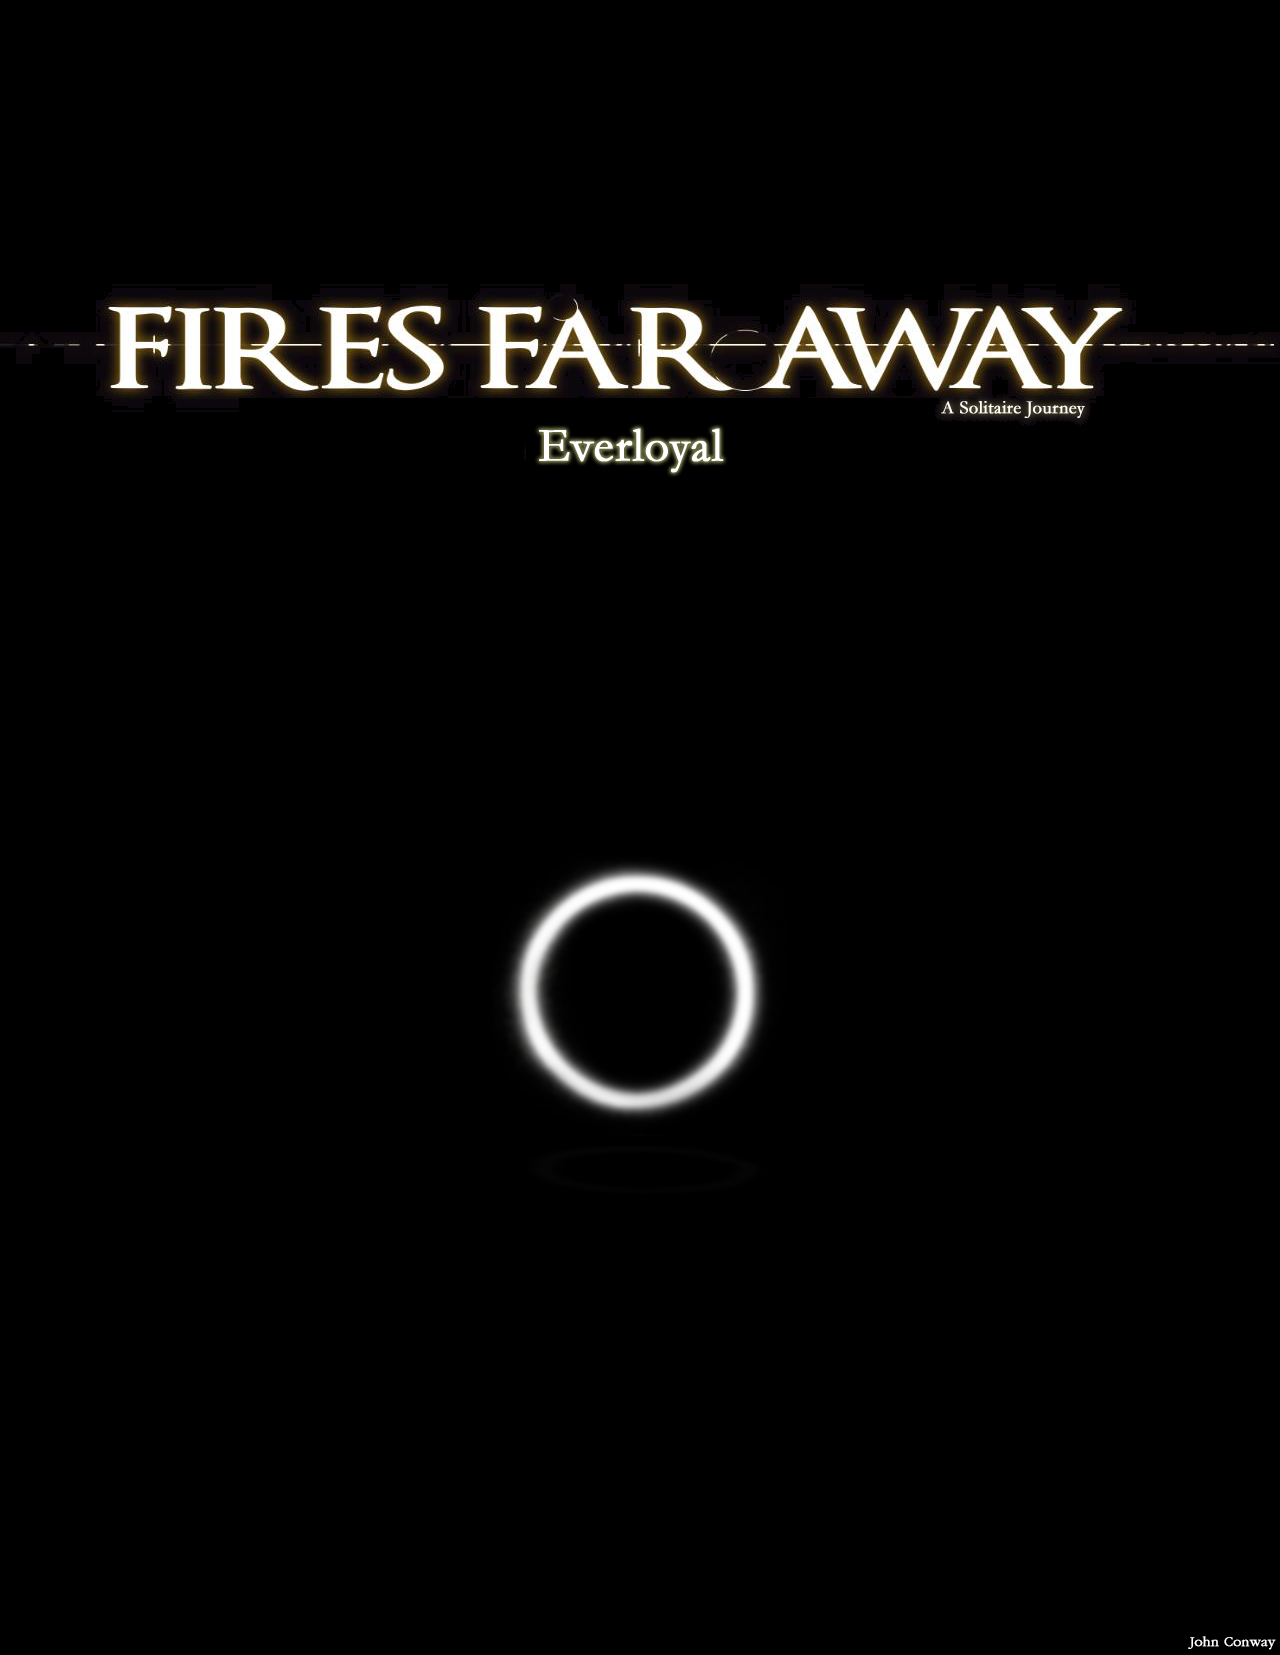
\includepdf{misc/cover.png}

\newpage

\vspace*{\fill}

\begin{center}
This page intentionally left blank.\\
\end{center}

\vspace*{\fill}

\pagebreak

\AddToShipoutPictureBG{
\includegraphics[width=\paperwidth,height=\paperheight]{misc/background.pdf}}

\phantomsection
\setlength\parindent{0pt}
\pagenumbering{arabic}
\setcounter{page}{1}

\begin{center}
\ \\
\ \\
\addcontentsline{toc}{section}{Introduction}
{\Huge GRAN  SELIDORE...}\\
\ \\
\ \\
\ \\
{\Large The Laurelled City\\
Brass Rose of the Vyl Coast\\
The Sheen of its Domed Towers now Dulled by\\
\textbf{Unabating Fog}\\
\ \\
Stripped of his Memories\\
Mankind Maunders as if Dreaming\\
With Emptied Eyes and\\
\textbf{Hollowed Souls}\\
\ \\
The Malediction\\
A Curse Laid Upon the Land\\
For the Failed Resurrection of a\\
\textbf{Dead God}\\
\ \\
Once-Risen and Twice-Slain\\
The King of all Secrets\\
Worshipped by the Forbidden Name of\\
\textbf{Av*rn-Z*l}\\
\ \\
Locked Away\\
In a Secluded Prison\\
Await Those who Bear the Sign of His...\\
\ \\
\ \\
{\Huge \textbf{E V E R L O Y A L}}\
}
\end{center}

\pagebreak

\begin{multicols*}{2}

\renewcommand*\contentsname{Table of Contents}
\hypersetup{hidelinks}
\tableofcontents
\addcontentsline{toc}{section}{Table of Contents}
\subsubsection*{And Attached Sheets...}
\vfill

\pagebreak

% DELETE BELOW %%%%%%%%%%%%%%%%%%%%%%%%%

\end{multicols*}

\vspace*{\fill}

\begin{center}
{\Large \textbf{Note:}
This is a playtest release that only includes the initial, tutorial chapter.\\
System mechanics and sections of the tutorial chapter will likely change in the final version.\\
}
\end{center}

\vspace*{\fill}

\pagebreak

\begin{multicols*}{2}

% DELETE ABOVE %%%%%%%%%%%%%%%%%%%%%%%%%

\section{Scenario}
\emph{Everloyal} is the companion scenario to be released alongside the first edition of \emph{Fires Far Away: A Solitaire Journey}. It is intended to be a player’s first experience with the system. Owing to this, the scenario contains an initial, tutorial chapter for easing players into the system as a whole. Other scenarios aren’t likely to implement a tutorial chapter unless they have significantly altered the system’s mechanics.

\subsection{Scenario Setup}
Ensure the following game materials are available:

\begin{itemize}
\item The corebook
\item Pencil(s) and an eraser
\item At least 8 six-sided dice
\item A pack of index cards or scratch paper
\item A bowl of coins, beads, or other small and discrete tokens (for damage, charges, etc)
\item Printed copies of the character, status, and record sheets (found at the end of this scenario book)
\item 3 double-sided copies of the Hexagon-Tiled Map (found at the back of the corebook)
\item Optionally: the encounter reference sheet (found at the back of the corebook)
\end{itemize}

Then complete the following steps:

\begin{enumerate}
\item Gather 6 blank index cards
\item Mark each card with one of the following chapter symbols: a \textbf{circle}; a \textbf{skull}; a domed \textbf{tower}; two crossed \textbf{arrows}; an \textbf{owl}; and an \textbf{eye} with a slit pupil 
\item Set the \textbf{circle} and \textbf{skull} cards aside
\item Shuffle the remaining 4 cards facedown
\item Place the \textbf{circle} card atop the deck, facedown
\end{enumerate}

Afterwards, the chapter deck should consist of four cards in random order, with the \textbf{circle} card on top and the \textbf{skull} card set aside.
\begin{tcolorbox}
\textbf{Note:} For this scenario, the \textbf{skull} chapter is not required to continue onto the \emph{prestige}.
\end{tcolorbox}
Once the game materials are gathered and the chapter deck is ready, it’s time to create a character.\\

\hyperlink{chargen}{\textbf{Turn to: Character Creation (Page \pageref{chargen}})}

\subsection{Scenario Resolution}
\label{scenres}\hypertarget{scenres}{}
After the character creation process is complete--and the character, record, and status sheets have been finalized-- begin drawing cards from the chapter deck and resolving their chapters.\\
To resolve a chapter, turn to its starting page (listed below). Continue through each chapter until the \textbf{End Chapter} instruction is encountered (either through victory over the chapter, or suffering a fatal defeat).\\
When the \textbf{End Chapter} instruction is encountered, erase all \emph{Ephemeral} items from the character sheet and stash. Next, clear any conditions and damage unless specifically instructed otherwise. Then erase any notes that are not bracketed by exclamation marks like: \emph{!!Note!!} Finally, draw the next chapter card and turn to its starting page.\\
After resolving the last card in the chapter deck, turn to the \emph{prestige’s} starting page for the scenario finale.\\
\ \\
\textbf{Chapter Starting Pages:}
\begin{itemize}
\item \textbf{Circle:} \hyperlink{c11}{Page \pageref{c11}:c11}
\item \textbf{Tower:} N/A %\hyperlink{t11}{Page \pageref{t11}:t11}
\item \textbf{Arrows:} N/A %\hyperlink{a11}{Page \pageref{a11}:a11}
\item \textbf{Owl:} N/A %\hyperlink{o11}{Page \pageref{o11}:o11}
\item \textbf{Eye:} N/A %\hyperlink{e11}{Page \pageref{e11}:e11}
\item \textbf{Skull:} N/A %\hyperlink{s11}{Page \pageref{s11}:s11}
\item \textbf{\emph{Prestige:}} N/A %\hyperlink{pres}{Page \pageref{pres}}
\end{itemize}

\begin{tcolorbox}
\textbf{Note:} Do not start reading sequentially through this scenario book and spoil yourself.
\end{tcolorbox}

\vspace*{\fill}
\pagebreak

\subsection{Scenario Concepts}
This section details gameplay concepts that are either unique to \emph{Everloyal} or have been significantly altered from the corebook. Reading this entire section is not necessary to begin play; simply reference these concepts as they’re encountered in-game.

\subsubsection{Chapters, Sections, and Readings}
Chapters are the main organizational unit of this scenario book. They refer to the six chapters of the game, each possessing its own chapter card. Every chapter has its own unique letter prepended to the codes of its readings and notes, i.e: \emph{c} for the \textbf{circle} chapter.\\
Chapters are broken into sections, which designate a general location within the chapter. The first number in the code for a reading designates its section, i.e: \emph{c1} for the first section of the \textbf{circle} chapter.\\
Readings are, as the name implies, the actual readings within a chapter. They are each designated by a code, prepended with its chapter and section serial, i.e: \emph{c11} for the first reading of the first section of the \textbf{circle} chapter.\\
Notes are named after the reading in which they are encountered, followed by a unique letter, i.e: \emph{c11a}.

\subsubsection{Conditions Roster}
\textbf{\emph{Cursed!:}} \hypertarget{Cursed!}{}\emph{Static.} Place the \textbf{skull} chapter card atop the chapter deck. The character immediately suffers a fatal defeat: \textbf{End Chapter.} The character loses all \refto{HMN} and souls, becomes Hollow, and cannot increase \refto{HMN} or upgrade \textbf{SL} while \reftoit{Cursed!} This condition can only be removed via a secret method (do not remove it while resolving \textbf{End Chapter}).\\

\textbf{Enhanced Defense:} \emph{Time-Limited - Round.} The entity’s specified \emph{sink} will increase by the listed amount while this condition is in effect.\\
The instructions for the enhanced \emph{sink} will look like: \textbf{P.DEF} (2), \textbf{F.DEF} (3), etc.\\
Try not to mistake the number of condition tokens for the Defense increase.\\
This condition is non-cumulative for each discrete \emph{sink}. The character sheet may not stack the effects of multiple Enhanced Defense tokens for a single \emph{sink}, but may benefit from multiple tokens affecting different \emph{sinks}.

\textbf{Enhanced Shield}: \emph{Time-Limited - Round.} The entity’s shield has all Durability restored, and gains bonus Defense and Stability.\\
The instructions for Defense and Stability increase will look like (1,2) respectively.\\
This condition is non-cumulative; ane ntity may only benefit from one Enhanced Shield token at a time.\\

\textbf{Enhanced Weapon:} \emph{Time-Limited - Round.} For the player, they will be asked to specify an equipped weapon. Attacks made by the specified weapon will deal additional damage while this condition is in effect. The amount and type of additional damage will be dictated by the source of this condition.\\
For enemies, the enemy sheet will specify the damage amount, type, as well as which attacks are enhanced.\\
The instructions for damage amount and type will look like: Poison (2), Burn (3), etc.\\
Try not to mistake the number of condition tokens for the damage increase.\\
The original damage inflicted by the weapon/attack retains its original damage type.\\
This condition is non-cumulative; the character may only benefit from one Enhanced Weapon token at a time.\\

\textbf{Mantra:} \emph{Static.} When the character is repeating a holy mantra, they gain a Mantra token on their status sheet that provides the mantra’s benefits. The status sheet is limited to a single Mantra token, which is replaced if the character activates a different mantra or is afflicted with Mute.\\

\textbf{Mute:} \emph{Time-Limited - Round.} A Mute entity cannot use any magic attacks or attunements, except for Guts and Revelations. When the character is inflicted with Mute, remove any Mystic Keys’ Mantra token from the status sheet.

\subsubsection{Fellows \& Tradables}
Trade is still alive and well in the fog-choked environs of Gran Selidore. Those few fellows who retain their sanity also retain their desire for barter--perhaps it’s essential to the well-being of the soul.\\
Fellows will part with the items, equipment, and attunements they’ve collected in exchange for tradables. Tradables can be anything from sweets to actual currency, and a fellow’s dedicated page will list their desires along with their offers (see the Fellows section for details).\\
Tradables can be \emph{Carried} and stored in the stash like any other equipment. Due to their small size, they can also be equipped in a pouch slot--and some tradables can even be used. If a tradable is used, then it is consumed as if it were an \emph{Ephemeral} item that had run out of charges. Tradables may also be “stacked” in their pouch or \emph{Carried} slot--mark how many tradables are held like: x1, x2, etc.\\
Of course, fellows are mortals and might be parted from their goods without the need for bartering--including those possessions they aren’t willing to trade away. But this kind of villainous behavior often has dire ramifications.

\subsubsection{Humanity, Memory, \& Hollowing}
\hypertarget{HMN}{}\hypertarget{MEM}{}
In \emph{Everloyal}, Humanity functions as a measure of the character’s memory. The character may mark \refto{HMN} boxes with acquired Humanity in the same manner described in the corebook. However, only \refto{HMN} boxes whose accompanying \reftoit{memento} (\refto{MEM}) slot is filled-in may be assigned Humanity.\\
When the player is instructed to lose Humanity, erase a \refto{HMN} box. If no \refto{HMN} boxes are marked, then \emph{erase the character’s name} and circle all permanent notes. If the character gains Humanity without possessing a name, then write a new, unique name for them instead of marking a \refto{HMN} slot.\\
A character without a name is considered Hollow (see the corebook’s Conditions Roster for details). Being Hollow during some events and chapter actions may alter their outcome.

\subsubsection{\emph{Mementos}}
\hypertarget{mementos}{}\hypertarget{memento}{}
Whenever the character acquires a \reftoit{memento}, fill-in the \refto{MEM} slot below a \refto{HMN} box. Filling-in this slot allows the accompanying \refto{HMN} box to be assigned with Humanity.\\
If the character loses or destroys one of their \reftoit{mementos}, erase a \refto{MEM} slot. Erasing the \refto{MEM} slot will not empty the accompanying \refto{HMN} box, it only prevents it from being marked again until another \reftoit{memento} is acquired.

\subsubsection{Names}
In \emph{Everloyal}, the character can forget their name by going Hollow. During hollowing, the player is instructed to erase their character’s name and circle all permanent notes. The circling of permanent notes designates them as experiences from a previous name. Some note checks might have further instructions depending on whether the character encountered them under a different name.\\
If a note check is bracketed like: \emph{(Note 123a)}, then the check requires that the note is \emph{not} circled.

\end{multicols*}
\pagebreak

\section{Character Creation}
\hbadness=99999
\label{chargen}
\hypertarget{chargen}{}
It is dark. A barred window casts a series of dim slivers onto the stone floor. The shadows of tiny, crawling things make their way along the illuminated mortar. You do not know where you are, or how you came to be here.\\
\emph{>> Begin with a score of 7 for each Primary Statistic on the character sheet.\\
>> Iterate through the steps of the character creation process in sequential order, altering the character sheet as instructed. Do not make any other alterations.}

\subsection*{Grasp at Your Fading Memories}
They slip through your conscious thoughts, leaving only the slight stain of their passing: those disconnected fragments that soon fade again like embers into a night sky. When you strain in recollection, what do you envision?\\
\emph{>> Select one option:}

\begin{multicols*}{2}
\subsubsection*{A Labyrinth of Streets}
Bare feet on cobblestone. People, but not faces. Smell of human refuse. Music and colored streamers. Cacophony of voices. Hunger.\\
\emph{>> DEX + 1; ATT + 1; VIT - 1 }

\subsubsection*{An Endless Weald}
Rain on a thatched roof. Wolves howling. Smell of split wood. Taste of mushrooms. Owl’s watchful eyes. Long walks with heavy loads. Fear.\\
\emph{>> END + 1; VIT + 1; ATT - 1 }

\subsubsection*{A Garden Terrace}
Saying the words; performing the motions. Haltering practice of chords. Stiff and sweltering costume. Taste of wine. Boredom.\\
\emph{>> INT + 1; DEX + 1; END - 1 }

\subsubsection*{An Idyllic Countryside}
Smell of pie: meat and greens. Goose honks; dog barks. Festival lanterns. Crunch of the trail. Cool water against the skin. Endless cavalcade of clouds.\\
\emph{>> VIT + 1; FTH + 1; INT - 1 }

\vspace*{\fill}
\columnbreak

\subsubsection*{A Vast Horizon}
Gulls squawking. Smell of fish. Pinch of sunburn. Clear days; storms. Sand underfoot. Aching palms. Rush of wind against the face.\\
\emph{>> FTH + 1; STR + 1; DEX - 1}

\subsubsection*{A Dour Swampland}
Smell of decay. Feet sloshing in soaked boots. Slight chill. Taste of eel and crayfish. Clinking of a pole lantern. Crackling fire. Haunting, distant calls.\\
\emph{>> ATT + 1; INT + 1; STR - 1 }

\subsubsection*{A Frigid Highland}
Bleating sheep. Creaking troika. Taste of mutton. Crunch of snow. Timeless vistas. Distant horns. Shivering cold.\\
\emph{>> STR + 1; END + 1; FTH - 1 }
\end{multicols*}

\subsection*{Examine Your Hands}
You hold your hands up to the faint light. There was skill in them once; you can almost feel them at work, even now. It’s as if they retain a memory all of their own. As they grasp and ungrasp, what do you recall?\\
\emph{>> Select one option:}

\begin{multicols*}{2}
\subsubsection*{A Well-Worn Pickaxe}
Pain. Time to work the left hand; give the right a little rest. No--still hurts there, too.\\
\emph{>> VIT + 2; END + 1; DEX - 1}

\subsubsection*{A Clenched Fist}
You punch it into your other hand, and wipe at your nose. Time to earn some coin.\\
\emph{>> END + 2; STR + 1; INT - 1}

\subsubsection*{A Wrapped \& Tarred Hilt}
The hilt jostles in your grip. One, two; one, two. Then suddenly, it isn’t a game anymore. The hilt shakes, despite your grip being tighter than ever before.\\
\emph{>> STR + 2; FTH + 1; ATT - 1}

\subsubsection*{A Lacquered Bow}
The string presses into your cheek. In your mind’s eye, you can see the arrow’s flight before it ever leaves your fingers.\\
\emph{>> DEX + 2; VIT + 1; STR - 1}

\subsubsection*{Playing Cards}
You lift the corners. Bad hand. Across the table, a mouth twitches. Bad hand. You shake your wrist a little. Good hand.\\
\emph{>> ATT + 2; DEX + 1; END - 1}

\subsubsection*{A Silver Goblet}
One hand pinches the stem, the other gesticulates. Emphasizing your words, circling the clever phrases. You are making your point quite clear.\\
\emph{>> INT + 2; ATT + 1; FTH - 1}

\subsubsection*{Sheep Entrails}
Lay them out. Poke them into place. Read carefully through the gore. There: an ill omen.\\
\emph{>> FTH + 2; INT + 1; VIT - 1}

\vfill
\columnbreak

\subsubsection*{A Wooden Yoke}
You pull. Stubborn bastard. You pull again. Damn it.\\
\emph{>> VIT + 2; STR + 1; ATT - 1}

\subsubsection*{Leather Reigns}
Another long ride--and hopefully, an uneventful one.\\
\emph{>> END + 2; VIT + 1; DEX - 1}

\subsubsection*{A Heavy Tool}
Clank of hammer; snore of saw. Smell of sawdust; heat of the forge. You squint to see your work clearer, and wipe the sweat from your brow.\\
\emph{>> STR + 2; DEX + 1; INT - 1}

\subsubsection*{A Hemp Rope}
Don’t look down. Almost there. You grab hold of the windowsill and pull yourself up. Once inside the darkened room, you carefully lower your sack to the floor.\\
\emph{>> DEX + 2; END + 1; VIT - 1}

\subsubsection*{A Marionette Paddle}
The manikin spins and dances. His face is all-too-familiar. The children might not catch the meaning now, but it will seep into their minds like a poison.\\
\emph{>> ATT + 2; INT + 1; FTH - 1}

\subsubsection*{An Owl Quill}
Your knuckles ache. You flex and unflex your hand, and grasp the quill again. Straining against the dim light, you carefully illustrate another vine entwined about the letter L.\\
\emph{>> INT + 2; FTH + 1; END - 1}

\subsubsection*{A Brass Chime}
Ring it once. Ring it again. Call them to you: the faithful, the curious, and especially the hecklers. They, most of all, must bear witness.\\
\emph{>> FTH + 2; ATT + 1; STR - 1}

\vfill
\end{multicols*}
\pagebreak

\subsection*{Collect Your Keepsake}
From above, there comes the pitter patter of droplets. A few pass through the barred window, and splash upon your cheeks. When the smell of petrichor strikes your senses, it stirs your failing memory to life.\\
Now you are pulling up the loose stone again--you are fishing out your treasure from the grit--you are cradling it in your weathered hands. This thing you hide so dearly: what is it?\\
\emph{>> Select one option:}

\begin{multicols}{2}
\subsubsection*{A Coin}
You pinch it by the rim, letting the light catch on its dull face. This coin is worth far more to you than its mere valuation.\\
\emph{>> STR + 1}

\subsubsection*{A Figurine}
You brush the dirt from the little figure’s face, like a tender parent might. It is so very important to keep it from weathering.\\
\emph{>> VIT + 1}

\subsubsection*{A Ring}
You slip it over your bony finger, then take it off again. It fits all the better as you grow more emaciated.\\
\emph{>> DEX + 1}

\subsubsection*{A Locket}
You pry it open, careful not to let any dirt fall inside, and risk a glance at the familiar likeness within.\\
\emph{>> END + 1}

\vspace*{\fill}
\columnbreak

\subsubsection*{A Fingerbone}
You lay it widthwise across your own bony fingers. The power that emanates from it is as strong as ever.\\
\emph{>> FTH + 1}

\subsubsection*{A Letter}
You clutch the decaying pages to your chest. Each reading of them feels fresh anew, thanks to your dwindling mind.\\
\emph{>> INT + 1}

\subsubsection*{A Fetish}
You hold it at length, as if it might bite you. A grotesque depiction, to be sure, but one you’re quite fond of.\\
\emph{>> ATT + 1}

\subsubsection*{A Pendant}
You hold the pendant up to the dim light. It’s quite possibly worthless--possibly.\\
\notegain{!!x11a!!} Possesses the pendant
\begin{tcolorbox}
\textbf{Note:} When a note is bracketed by !!, it is a permanent note, and is not erased during \textbf{End Chapter} actions.
\end{tcolorbox}
\end{multicols}
\hrule
\ \\
\ \\
Whatever meaning this keepsake holds, only you can say. But whether that memory is merely the product of a fragmented mind, not even its keeper could ever truly be certain.\\
\emph{>> Fill-in the first \refto{MEM} box on the character sheet for your personal memento\\
>> Fill-in the first \refto{HMN} slot}
\begin{tcolorbox}
\textbf{Note:} In \emph{Everloyal}, the character’s maximum \refto{HMN} is determined by their number of \reftoit{mementos}. Each acquired \reftoit{memento} marks a \refto{MEM} box, which enables its accompanying \refto{HMN} slot to hold Humanity.\\
When the character gains or loses Humanity, an available \refto{HMN} slot is filled-in or erased.\\
A \refto{MEM} box only loses its mark if the character loses or destroys the accompanying \reftoit{memento}.
\end{tcolorbox}

\subsection*{Ruminate on the Pain}
As you cradle your treasure, the damp air reignites a nostalgic sting; a hurting from somewhere deep in the remote histories of your past. From whence it came, you do not know, but it dutifully reminds you of its presence time and again. This old pain that’s surfaced now: what wounds you?\\
\emph{>> Select one option:}

\begin{multicols}{2}
\subsubsection*{Chronic Fever}
You turn your face up to the rain, and wipe its droplets across your brow. It helps cool the fever--but not by much.\\
\emph{>> VIT - 1; Any Primary Stat + 1}

\subsubsection*{Wracked Lungs}
You cough and convulse, but to no avail. For a moment, it feels as though you might drown on dry land.\\
\emph{>> END - 1; Any Primary Stat + 1}

\subsubsection*{Wasting Illness}
You drag an arm across the stone floor, and lay it in your lap. It’s fallen asleep again, and soon feels as though you’d plunged it into a nest of hornets.\\
\emph{>> STR - 1; Any Primary Stat + 1}

\subsubsection*{A Missing Eye}
You poke a finger into the hole that once held your eye. Wherever did it go?\\
\emph{>> DEX - 1; Any Primary Stat + 1}

\vspace*{\fill}
\columnbreak

\subsubsection*{A Maimed Hand}
You are missing a number of fingers from one hand. Funny how it feels as if they’re still there.\\
\emph{>> ATT - 1; Any Primary Stat + 1}

\subsubsection*{Splitting Headaches}
They’ve started again. You bury your eyes in your palms and wait for them to pass.\\
\emph{>> INT - 1; Any Primary Stat + 1}

\subsubsection*{Mutilated Genitalia}
O, right--\emph{that}.\\
\emph{>> FTH - 1; Any Primary Stat + 1}

\subsubsection*{Scars}
They criss cross your body like the lattices of a fisherman’s net. All from one source, or the accumulation of years?\\
\emph{>> No changes}\\
\end{multicols}
\hrule
\ \\
\ \\
Then suddenly the light is gone, taking all earthly sense with it. You feel yourself slipping: down to starless skies of madness. How many times have you repeated this labor? Finding and losing; forgetting and remembering and then forgetting again. No! You reach for something--anything to latch onto.

\subsection*{Try to Remember Your Name}
What was it? It should be so simple, and yet...\\

As a necessity of your vocation, you have had many. They march across your tongue to a familiar cadence, but you cannot discern the original from its phalanx of impostors. Out of desperation, you whisper one to yourself. What is it?\\
\emph{>> Write a name on the character sheet}

\pagebreak

\subsection*{Affirm Your Purpose}
You once again teeter on the precipice of nothingness: rocking back and forth, clutching your keepsake to your heart, and repeating that glib moniker to yourself like a mantra. It is a futile effort. You will forget as you have innumerable times before. And perhaps you will remember yourself again, or maybe you conjure up a new identity with each bout of clarity--like some ironic punishment for your life’s work: that web of lies and misdeeds...\\
\ \\
For there is one facet of yourself which you could never forget. Etched into your skin: your very purpose within this mortal coil. You trace the Sign with a finger. It is your light and your anchor; the flotsam you cling to in this capsized world...\\
\emph{>> Mark SL as 5\\
>> Calculate all Distributory Values\\
>> Finalize the status sheet}

\begin{center}
\vspace*{\fill}
{\Large
Once-Risen and Twice-Slain\\
The Black and Golden Key\\
King of all Secrets\\
\textbf{Av*rn-Z*l}\\
\ \\
His Faithful Gather in Furtive Circles\\
They Know Their kin by His Sign\\
And the Promise That was Made:\\
He Walked This World Once, and Shall Walk Again...\\
\ \\
\ \\
{\Huge \textbf{E V E R L O Y A L }}
}
\vspace*{\fill}
\end{center}

\hyperlink{scenres}{\textbf{Turn to: Scenario Resolution (Page \pageref{scenres}})}

\section{Chapters}

\subsection{The Circle}

%C1%

\chapsection{c1}{1}{Locked Away}

\chapsection{c1}{3}{Row of Cells}

\encountersection{c1}{2}{The Jailer}

\chapsection{c1}{5}{Jailer’s Office}

\chapsection{c1}{4x1}{Stuck}

\chapsection{c1}{6}{The Green Door}

\chapsection{c1}{5x2}{Not Squeamish}

\chapsection{c1}{7}{Ratfriend Niki}

\chapsection{c1}{4}{Large, Iron-Barred Doors}

\chapsection{c1}{5x1}{Gruesome Discovery}

\chapsection{c1}{6x1}{Strappado}

\chapsection{c1}{7x2}{A Gentler Method}

\chapsection{c1}{7x1}{Smash-smash}

\chapsection{c1}{6x2}{Strappado (Broken Window)}

\chapsection{c1}{4x2}{The Supple Ratfriend}

\chapsection{c1}{8}{A Debt Repaid}

\chapsection{c1}{5x3}{Desperate Measures}

\encountersection{c1}{9}{Mad Bedfellows}

%C2%

\chapsection{c2}{12x6}{Ending the Nightmare}

\chapsection{c2}{1}{Central Mezzanine}

\chapsection{c2}{7}{Niche}

\chapsection{c2}{12x3}{Twinkling Drain}

\chapsection{c2}{5}{Collapsed Stairwell}

\chapsection{c2}{9}{Half-Hidden Door}

\chapsection{c2}{10x3}{The Reward}

\chapsection{c2}{4}{Rubble-Strewn Corridor}

\chapsection{c2}{1x1}{Mezzanine Cells}

\chapsection{c2}{3}{Mezzanine Corridor}

\chapsection{c2}{6}{Crumbling Walkway}

\chapsection{c2}{10x1}{Solution of Strength}

\chapsection{c2}{9x1}{Behind the Half-Hidden Door}

\chapsection{c2}{8}{Fog-Stricken Passage}

\chapsection{c2}{11}{Raised Walkway}

\chapsection{c2}{12x2}{A Familiar Face}

\chapsection{c2}{2}{Mezzanine Balcony}

\chapsection{c2}{10}{Looted Armory}

\chapsection{c2}{10x2}{Solution of Wits}

\chapsection{c2}{12x1}{Hygiene Processing Room}

\chapsection{c2}{5x1}{A Sprig of Queergrass}

\chapsection{c2}{1x3}{Back for More}

\chapsection{c2}{1x2}{The Borrowed Blade}

\chapsection{c2}{12x5}{Battle Without Honor and Humanity}

\chapsection{c2}{12x4}{The Second Encounter}

\chapsection{c2}{13}{Common Area Entryway}

\encountersection{c2}{14}{The Lost Phalanx}

\chapsection{c2}{16}{The Cellmates}

\chapsection{c2}{18}{Security Hallway}

\chapsection{c2}{17}{Cell Block Main Doors}

\chapsection{c2}{16x1}{Free Men}

\chapsection{c2}{15}{Cell Block Yard}

\chapsection{c2}{18x2}{The Memento}

\chapsection{c2}{17x1}{The Sinecure-Holder and the Vagabond}

\chapsection{c2}{18x1}{Contraband}

%C3/C4%

\chapsection{c3}{2}{Barricaded Entrance}

\chapsection{c3}{3x1}{A Wrought Iron Gate}

\chapsection{c3}{8x2}{Felled Giant}

\chapsection{c3}{16x3}{One Unlike the Others}

\chapsection{c3}{1}{Rotunda}

\chapsection{c3}{7x3}{A Powerful Substance}

\chapsection{c3}{6x9}{The Academic's Offer}

\chapsection{c3}{2x1}{New Threads}

\chapsection{c3}{5x1}{Incinerated Contraband Lockers}

\chapsection{c3}{6x14}{A Gnostic's Ink}

\chapsection{c3}{6x1}{Vagabond Lor}

\chapsection{c3}{2x2}{A Perilous Climb}

\chapsection{c3}{3}{Beneath the Rotunda}

\chapsection{c3}{4x1}{Rotunda Balcony}

\chapsection{c3}{6}{The Everloyal}

\chapsection{c3}{14}{Blasted Yard}

\chapsection{c3}{5x2}{Strange Powder}

\chapsection{c3}{8x1}{The Infirmary}

\chapsection{c3}{12x3}{Amateur Studies}

\chapsection{c3}{8}{Bloody Hallway}

\chapsection{c3}{6x3}{Ratfriend Niki}

\chapsection{c3}{6x15}{Enchantment}

\chapsection{c3}{3x2}{Ominous Portents}

\chapsection{c3}{7}{Complex Halls}

\chapsection{c3}{6x13}{A Letter of Power}

\chapsection{c3}{5}{Scorched Security Hallway}

\chapsection{c3}{6x4}{Zealot Eóghainn}

\chapsection{c3}{10x1}{Armored Dummy}

\chapsection{c3}{3x3}{The Late Warden}

\chapsection{c3}{6x10}{Beneath the Crawlspace}

\chapsection{c4}{4}{Spoils}

\chapsection{c3}{12x1}{Looting the Cubicles}

\chapsection{c3}{3x5}{A Gathering of Faithful}

\chapsection{c3}{3x4}{The Warden’s Key}

\chapsection{c3}{6x2}{Sinecure Petanti}

\chapsection{c3}{6x7}{The Gift of Fire}

\chapsection{c3}{13x1}{That Unforgettable Insult}

\chapsection{c3}{4}{Rotunda, Second Floor}

\chapsection{c3}{6x5}{Annalist "Littletongue" Astrid}

\encountersection{c3}{11}{Goldhand Heist Remnants}

\chapsection{c3}{6x6}{Vile Acts}

\chapsection{c3}{7x2}{Muscle Memory}

\chapsection{c3}{9}{Looted Armory Entrance}

\chapsection{c4}{1x3}{Terse Introductions}

\chapsection{c3}{6x8}{Sorcerous Studies}

\chapsection{c3}{12}{Back Offices}

\chapsection{c3}{24x1}{Panicked Flight}

\chapsection{c3}{23x2}{For All Mankind}

\chapsection{c4}{1}{Underground Dock}

\chapsection{c3}{13}{Mess Hall}

\chapsection{c3}{6x11}{The Mystic Keys}

\chapsection{c3}{18}{Desolate Hygiene Room}

\chapsection{c3}{16}{Exposed Mezzanine}

\chapsection{c3}{22x3}{King of the Woods}

\chapsection{c3}{27x3}{The Dice Game}

\encountersection{c3}{15}{Lukso the Metamorphosed}

\chapsection{c3}{6x12}{The Zealot's Offer}

\chapsection{c3}{6x16}{Floor Plans}

\chapsection{c3}{19x1}{A Leap of Faith}

\chapsection{c3}{17x2}{Take Me to Them}

\chapsection{c3}{8x3}{Queergrass Poultice}

\chapsection{c4}{3x1}{Payment Due}

\chapsection{c3}{6x17}{Secrets Within Secrets}

\chapsection{c3}{6x19}{A Helping Hand}

\chapsection{c4}{1x2}{The Hired Blade}

\chapsection{c3}{6x18}{Champion}

\chapsection{c3}{8x4}{Mercy}

\chapsection{c4}{3}{Goldhand Jacquelyn}

\chapsection{c3}{25}{An Unexpected Find}

\chapsection{c3}{7x1}{Tidy Office}

\chapsection{c3}{12x2}{Bottled Moonlight}

\chapsection{c3}{27x2}{Looting the Barracks}

\chapsection{c3}{10}{Destroyed Armory}

\chapsection{c3}{6x20}{Embarrassment}

\chapsection{c3}{11x1}{A Friendly Snout}

\chapsection{c3}{23}{Kitchen}

\chapsection{c4}{1x1}{The Beast, Slain}

\chapsection{c3}{16x1}{Windswept Precipice}

\chapsection{c3}{27}{Guards' Barracks}

\chapsection{c3}{21}{Warden's Door}

\chapsection{c3}{13x2}{The Hunt}

\encountersection{c3}{17}{The Zealot’s Trial}

\chapsection{c3}{16x2}{A Nest of Corpses}

\chapsection{c3}{17x1}{The Trial's Conclusion}

\chapsection{c4}{5}{Supply Crates}

\chapsection{c3}{17x3}{A Man of Righteous Intent}

\chapsection{c3}{27x4}{Faulty Locks}

\chapsection{c3}{26}{Battered Iron Door}

\chapsection{c3}{19}{Narrow Walkway}

\chapsection{c3}{22x1}{Hidden Cache}

\chapsection{c3}{23x1}{No Friend of Yours}

\chapsection{c3}{22}{Warden's Office}

\chapsection{c3}{24}{Minaret Stairwell}

\chapsection{c3}{22x2}{The Warden’s Hobby}

\chapsection{c3}{25x1}{Littletongue}

\chapsection{c3}{27x1}{Prison Cliffside}

\chapsection{c3}{11x2}{Cramped Quarters}

\encountersection{c3}{20}{The Beast from the Fog}

\chapsection{c4}{2}{The Mad Crusade}


\pagebreak

\section{Fellows}

\makefellow{Ratfriend Niki (Circle)}

\pagebreak

\renewcommand{\arraystretch}{1.5}
\definecolor{Gray}{gray}{0.85}
\rowcolors{1}{Gray}{}

\subsection{Weapons}
\subsubsection*{Weapon Anatomy}
\begin{itemize}
\item \textbf{Weapon:} Self-explanatory
\item \textbf{SP:} The \textbf{SP} score required to attack with this weapon
\item \textbf{Dam:} Base damage, and types of damage available (X means all three: Slash, Crush, and Pierce)
\item \textbf{Wt:} Weight of the weapon (always in effect, regardless of whether it’s currently held)
\item \textbf{Hd:} Whether the weapon is one-handed or two-handed by default
\item \textbf{Rg:} The maximum range of the weapon in tiles
\item \textbf{Dur:} Durability \emph{sinks} on the weapon, if any
\item The requirements for each Primary Stat, followed by their scaling grade
\item \textbf{S.Attacks:} Any special attacks enabled for the weapon
\item Any additional notes on the weapon
\end{itemize}

\subsubsection*{Weapons Roster}
\begin{center}
\begin{tabularx}{\textwidth}{p{0.12\textwidth}p{0.023\textwidth}p{0.054\textwidth}p{0.024\textwidth}p{0.024\textwidth}p{0.03\textwidth}p{0.03\textwidth}p{0.12\textwidth}p{0.11\textwidth}p{0.23\textwidth}}
\hline
\rowcolor{white} \multicolumn{10}{l}{\textbf{Daggers \& Knives}}\\
\hline
\rowcolor{white} \textbf{Weapon} & \textbf{SP} & \textbf{Dam} & \textbf{Wt} & \textbf{Hd} & \textbf{Rg} & \textbf{Dur} & \textbf{Stat Reqs} & \textbf{S.Attacks} & \textbf{Notes}\\
\hline
\makeitem{Fighting Knife} & 1 & 1 S,P & 1 & 1H & 1 & 1 & STR - 3|D\newline DEX - 3|D & Backstab & Coup De Grâce \textbf{SP} cost is reduced to Wep\\
\makeitem{Knife} & 1 & 1 S,P & 1 & 1H & 1 & - & STR - 3|D\newline DEX - 3|D & Backstab & Coup De Grâce \textbf{SP} cost is reduced to Wep\\
\makeitem{Main-Gauche} & 1 & 1 P & 1H & 1 & 1 & - & STR - 5|D\newline DEX - 10|B & N/A & Coup De Grâce \textbf{SP} cost is reduced to Wep\newline Parry-like actions can use \textbf{SP} dice 1 score higher than the target die (only if this weapon is currently held)\\
\makeitem{Seax} & 1 & 1 S,P & 1 & 1H & 1 & 1 & STR - 4|D\newline DEX - 6|B & Cut, Lunge & Coup De Grâce \textbf{SP} cost is reduced to Wep\\
\makeitem{Stiletto} & 1 & 1 P & 1 & 1H & 1 & - & STR - 3|D\newline DEX - 9|B & Backstab, Lunge, Puncture & Coup De Grâce \textbf{SP} cost is reduced to Wep\\
\hline
\end{tabularx}
\end{center}

\begin{center}
\begin{tabularx}{\textwidth}{p{0.12\textwidth}p{0.023\textwidth}p{0.054\textwidth}p{0.024\textwidth}p{0.024\textwidth}p{0.03\textwidth}p{0.03\textwidth}p{0.12\textwidth}p{0.11\textwidth}p{0.23\textwidth}}
\hline
\rowcolor{white} \textbf{Weapon} & \textbf{SP} & \textbf{Dam} & \textbf{Wt} & \textbf{Hd} & \textbf{Rg} & \textbf{Dur} & \textbf{Stat Reqs} & \textbf{S.Attacks} & \textbf{Notes}\\
\hline
\rowcolor{white} \multicolumn{10}{l}{\textbf{Swords}}\\
\hline
\makeitem{Broadsword} & 2 & 2 S,P & 2 & 1H & 1 & 1 & STR - 7|C\newline DEX - 7|C & Cut & N/A \\
\makeitem{Broken Shortsword} & 2 & 2 S,P & 1 & 1H & 1 & - & STR - 5|D\newline DEX - 5|D & N/A & Deals -1 damage for Pierce attacks\\
\makeitem{Claymore} & 3 & 4 S,P & 3 & 2H & 1 & 2 & STR - 10|B\newline DEX - 7|C & Lunge & Pierce attacks are range 2\\
\makeitem{Saber} & 2 & 2 S,P & 2 & 1H & 1 & 1 & STR - 7|C\newline DEX - 10|B & Cut, Fend & N/A \\
\makeitem{Shortsword} & 2 & 2 S,P & 2 & 1H & 1 & 1 & STR - 7|C\newline DEX - 7|C & Flurry & N/A\\
\hline
\rowcolor{white} \multicolumn{10}{l}{\textbf{Bludgeons}}\\
\hline
\makeitem{Truncheon} & 1 & 1 C & 1 & 1H & 1 & - & STR - 4|D\newline DEX - 3|D & N/A & N/A\\
\makeitem{Mace} & 3 & 3 C & 2 & 1H & 1 & - & STR - 9|B\newline DEX - 4|D & N/A & Cannot be Broken\\
\hline
\rowcolor{white} \multicolumn{10}{l}{\textbf{Polearms}}\\
\hline
\makeitem{Halberd} & 4 & 5 S,P & 3 & 2H & 2 & 1 & STR - 13|A\newline DEX - 8|C & N/A & Sweep \textbf{SP} cost is reduced to Wep+1\newline Spin \textbf{SP} cost is reduced to Wep+2\\
\makeitem{Makeshift Spear} & 1 & 1 P & 1 & 1H & 2 & - & STR - 5|D\newline DEX - 5|D & N/A & N/A\\
\makeitem{Spear} & 2 & 2 P & 2 & 2H & 2 & 1 & STR - 7|C\newline DEX - 7|C & N/A & N/A\\
\makeitem{Warped Spear} & 2 & 2 P & 2 & 1H & 2 & - & STR - 6|D\newline DEX - 6|D & N/A & N/A\\
\hline
\rowcolor{white} \multicolumn{10}{l}{\textbf{Axes}}\\
\hline
\makeitem{Axe} & 2 & 2 S & 2 & 1H & 1 & 1 & STR - 8|C\newline DEX - 6|D & Shieldbreak & N/A\\
\makeitem{Battleaxe} & 3 & 3 S & 3 & 1H & 1 & 1 & STR - 10|B\newline DEX - 7|D & Shieldbreak & Cleave \textbf{SP} cost is reduced to Wep\\
\hline
\end{tabularx}
\end{center}

\begin{center}
\begin{tabularx}{\textwidth}{p{0.12\textwidth}p{0.023\textwidth}p{0.054\textwidth}p{0.024\textwidth}p{0.024\textwidth}p{0.03\textwidth}p{0.03\textwidth}p{0.12\textwidth}p{0.11\textwidth}p{0.23\textwidth}}
\hline
\rowcolor{white} \textbf{Weapon} & \textbf{SP} & \textbf{Dam} & \textbf{Wt} & \textbf{Hd} & \textbf{Rg} & \textbf{Dur} & \textbf{Stat Reqs} & \textbf{S.Attacks} & \textbf{Notes}\\
\hline
\rowcolor{white} \multicolumn{10}{l}{\textbf{Ranged Weaponry}}\\
\hline
\makeitem{Hand Crossbow} & 1 & 1 & 1 & 1H & 5 & 1 & STR - 6|E\newline DEX - 7|C\newline INT - 6|E & N/A & Loadable ranged weapon\newline Damage type dependent on missile (uses bolts)\newline Can commit Shoot one-handed\\
\makeitem{Light Crossbow} & 1 & 1 & 2 & 2H & 7 & 1 & STR - 8|E\newline DEX - 8|C\newline INT - 6|E & N/A & Loadable ranged weapon\newline Damage type dependent on missile (uses bolts)\\
\makeitem{Shortbow} & 2 & - & 1 & 2H & 2-5 & - & STR - 5|D\newline DEX - 6|C & N/A & Ranged weapon\newline Damage and damage type dependent on missile (uses arrows)\\
\hline
\rowcolor{white} \multicolumn{10}{l}{\textbf{Special Weapons}}\\
\hline
\makeitem{Fist} & 2 & 1 C & - & 1H & 1 & - & N/A & N/A & Cannot be Broken\newline Use if nothing else is equipped\newline Increases damage by 1 at 14 \textbf{STR} and 22 \textbf{STR}\newline No 2H\\
\makeitem{Loose Cobblestone} & 1 & 1 C & - & 1H & 1 & - & STR - 3|D\newline DEX - 3|E & N/A & \emph{Ephemeral}\newline Cannot be Broken\newline No 2H\\
\makeitem{Meat Hook} & 1 & 1 P & 1 & 1H & 1 & - & STR - 3|D\newline DEX - 4|D & Defeat Guard & Coup De Grâce \textbf{SP} cost is reduced to Wep\\
\makeitem{Sock Full of Rocks} & 1 & 1 C & - & 1H & 1 & - & STR - 3|D\newline DEX - 4|D & Defeat Guard & \emph{Ephemeral}\newline Overhead deals +1 damage\\
\makeitem{Torch} & 1 & 1 C & 1 & 1H & 1 & - & N/A & Light/Douse,\newline Set Aflame &  Must be lit to use Set Aflame\newline Counts as a light source when lit\\
\makeitem{Whip} & 2 & 1 S & 1 & 1H & 2-3 & - & STR - 4|E\newline DEX - 8|C & Defeat Guard, Pull & If this weapon assigns any damage to \textbf{HP} slots in a single attack, it also inflicts 1 Bleed\newline Cannot commit Parry or Coup De Grâce\\
\hline
\end{tabularx}
\end{center}

\begin{center}
\begin{tabularx}{\textwidth}{p{0.12\textwidth}p{0.023\textwidth}p{0.054\textwidth}p{0.024\textwidth}p{0.024\textwidth}p{0.03\textwidth}p{0.03\textwidth}p{0.12\textwidth}p{0.11\textwidth}p{0.23\textwidth}}
\hline
\rowcolor{white} \textbf{Weapon} & \textbf{SP} & \textbf{Dam} & \textbf{Wt} & \textbf{Hd} & \textbf{Rg} & \textbf{Dur} & \textbf{Stat Reqs} & \textbf{S.Attacks} & \textbf{Notes}\\
\hline
\rowcolor{white} \multicolumn{10}{l}{\textbf{Unique Weapons}}\\
\hline
\makeitem{Lucky Razor} & 1 & 1 S & 1 & 1H & 1 & - & STR - 3|D\newline DEX - 3|D & Backstab & While equipped, immediately after rolling the \emph{stamina pool} the character may re-roll 1 \textbf{SP} Die. Remember that re-rolls are once-per-die and the second result is final.\newline Coup De Grâce \textbf{SP} cost is reduced to Wep \\
\hline
\end{tabularx}
\end{center}

\pagebreak

\subsection{Shields}
\subsubsection*{Shield Anatomy}
\begin{itemize}
\item \textbf{Shield:} Self-explanatory
\item \textbf{Stab:} The Stability of the shield, or how many damage tokens it can block before suffering \emph{Guard Break}
\item \textbf{Def:} How much damage the shield can block from a single attack; also determines the \textbf{SP} cost of \emph{Shield Up!}
\item \textbf{Dam:} Damage inflicted by using the shield as a weapon
\item \textbf{Wt:} Weight of the shield (always in effect, regardless of whether it’s currently held)
\item \textbf{Dur:} Durability \emph{sinks} on the shield, if any
\item The requirements for each Primary Stat
\item \textbf{S.Attacks:} Any special attacks enabled for the shield
\item Any additional notes on the shield
\end{itemize}

\subsubsection*{Shields Roster}
\begin{center}
\begin{tabularx}{\textwidth}{p{0.15\textwidth}p{0.03\textwidth}p{0.035\textwidth}p{0.035\textwidth}p{0.024\textwidth}p{0.03\textwidth}p{0.12\textwidth}p{0.12\textwidth}p{0.245\textwidth}}
\hline
\rowcolor{white} \textbf{Shield} & \textbf{Def} & \textbf{Stab} & \textbf{Dam} & \textbf{Wt} & \textbf{Dur} & \textbf{Stat Reqs} & \textbf{S.Attacks} & \textbf{Notes}\setcounter{rownum}{0}\\
\hline
\makeitem{Battered Kite Shield} & 2 & 5 & 1 C & 2 & - & STR - 7 & N/A & N/A\\
\makeitem{Buckler} & 1 & 4 & 1 C & 1 & 1 & STR - 6\newline DEX - 9 & Riposte & N/A\\
\makeitem{Cracked Round Shield} & 1 & 4 & 1 C & 1 & - & STR - 5 & N/A & N/A\\
\makeitem{Kite Shield} & 2 & 6 & 1 C & 2 & 1 & STR - 7 & N/A & N/A\\
\makeitem{Round Shield} & 2 & 5 & 1 C & 3 & 1 & STR - 8 & N/A & Do not place blocked damage tokens from non-\emph{Magical} ranged attacks on \emph{Shield Up!}\\
\makeitem{Table Shield} & 1 & 5 & 1 C & 2 & 1 & STR - 6 & N/A & N/A\\
\hline
\end{tabularx}
\end{center}

\pagebreak

\subsection{Armor \& Outfits}
\subsubsection*{Armor \& Outfit Anatomy}
\begin{itemize}
\item \textbf{Set:} Self-explanatory
\item \textbf{Def:} How much \textbf{P.DEF} is increased by equipping the set
\item \textbf{PS:} How much \textbf{PS} is increased by equipping the set
\item \textbf{Wt:} Weight of the set when equipped
\item \textbf{Dur:} Durability \emph{sinks} on this equipment, if any
\item The requirements for each Primary Stat
\item Any additional notes on the set
\end{itemize}

\subsubsection*{Armor \& Outfits Roster}
\begin{center}
\begin{tabularx}{\textwidth}{p{0.2\textwidth}p{0.035\textwidth}p{0.035\textwidth}p{0.035\textwidth}p{0.035\textwidth}p{0.12\textwidth}p{0.38\textwidth}}
\hline
\rowcolor{white} \textbf{Set} & \textbf{Def} & \textbf{PS} & \textbf{Wt} & \textbf{Dur} & \textbf{Stat Reqs} & \textbf{Notes}\setcounter{rownum}{0}\\
\hline
\makeitem{Prisoner’s Chains} & - & - & 3 & - & N/A & Reduces \textbf{END} by 2 when equipped \\
\makeitem{Threadbare Guard’s Set} & 1 & - & 3 & - & STR - 6\newline DEX - 4 & N/A \\
\hline
\end{tabularx}
\end{center}

\pagebreak

\subsection{Catalysts}
\subsubsection*{Catalyst Anatomy}
\begin{itemize}
\item \textbf{Catalyst:} Self-explanatory
\item \textbf{Type(s):} What attunement type(s) the catalyst enables
\item \textbf{PWR:} Base \textbf{PWR} of attunements cast with the catalyst
\item \textbf{Dam:} Damage inflicted by using the catalyst as a weapon. All catalysts are \textbf{SP} 2 unless stated otherwise
\item \textbf{Wt:} Weight of the catalyst (always in effect, regardless of whether it’s currently held)
\item \textbf{Dur:} Durability \emph{sinks} on this equipment, if any
\item The requirements for each Primary Stat
\item \textbf{S.Attacks:} Any special attacks enabled for the catalyst
\item Any additional notes on the catalyst
\end{itemize}
\emph{All catalysts are assumed to be one-handed unless stated otherwise}

\subsubsection*{Catalysts Roster}
\begin{center}
\begin{tabularx}{\textwidth}{p{0.12\textwidth}p{0.11\textwidth}p{0.05\textwidth}p{0.04\textwidth}p{0.02\textwidth}p{0.03\textwidth}p{0.12\textwidth}p{0.1\textwidth}p{0.2\textwidth}}
\hline
\rowcolor{white} \textbf{Catalyst} & \textbf{Type(s)} & \textbf{PWR} & \textbf{Dam} & \textbf{Wt} & \textbf{Dur} & \textbf{Stat Reqs} & \textbf{S.Attacks} & \textbf{Notes}\setcounter{rownum}{0}\\
\hline
\makeitem{Crude Wand} & Invocations & 0 & 1 C & - & - & INT - 10 & N/A & N/A\\
\makeitem{Ornate Wand} & Invocations & 1 & 1 C & - & - & INT - 10 & N/A & N/A\\
\makeitem{Eternal Ember} & Pyromancy & 1* & 1 B & - & - & - & Set Aflame & Can never be doused, and never needs to be lit\newline *This catalyst’s \textbf{PWR} can be upgraded in-game\\
\makeitem{Secret Calligraphy} & Secrets \& Revelations & 1 & - & - & - & FTH - 10 & N/A & N/A\\
\hline
\end{tabularx}
\end{center}

\pagebreak

\subsection{Rings}
\subsubsection*{Rings Anatomy}
\begin{itemize}
\item \textbf{Ring:} Self-explanatory
\item \textbf{Effects:} Effects produced by equipping the ring
\end{itemize}

\subsubsection*{Rings Roster}
\begin{center}
\begin{tabularx}{\textwidth}{p{0.3\textwidth}p{0.65\textwidth}}
\hline
\rowcolor{white} \textbf{Ring} & \textbf{Effects}\setcounter{rownum}{0}\\
\hline
\makeitem{Babygold Ring} & Increase \textbf{EQP} by 1 \\
\makeitem{Bloodstone Ring} & Increase \textbf{RES} by 1 \\
\makeitem{Charcoal Ring} & Retains 2 Durability slots \\
\makeitem{Lover Hair Ring} & Increase \textbf{HP} by 1 \\
\makeitem{Ornate Gold Ring} & Increase \textbf{POTs} by 1 \\
\makeitem{Silver Ring} & Increase \textbf{FP} by 1 \\
\makeitem{Rat Tail Ring} & Increase \textbf{EQP} and \textbf{RES} by 1 each \\
\makeitem{Ring of Favor} & Increase \textbf{HP}, \textbf{FP}, and \textbf{EQP} by 1 each. Once unequipped, erase this ring as if it were \emph{Ephemeral} \\
\makeitem{Tearstone Ring} & When the character would lose \textbf{HMN}, erase this ring from the character sheet instead \\
\makeitem{Twisted Ring} & After resolving the effects of Bleeding during a Turn, remove 1 Bleeding condition token from the character sheet\\
\hline
\end{tabularx}
\end{center}

\pagebreak

\subsection{Flasks}
\subsubsection*{Flasks Anatomy}
\begin{itemize}
\item \textbf{Flask:} Self-explanatory
\item \textbf{Charges:} Number of uses a flask contains. Recharged during \emph{short reprieves}
\item \textbf{E?} Whether the flask is \emph{Ephemeral}
\item \textbf{Effects:} Effects produced by drinking from the flask
\end{itemize}

\subsubsection*{Flasks Roster}
\begin{center}
\begin{tabularx}{\textwidth}{p{0.2\textwidth}p{0.1\textwidth}p{0.1\textwidth}p{0.505\textwidth}}
\hline
\rowcolor{white} \textbf{Flask} & \textbf{Charges} & \textbf{E?} & \textbf{Effects}\setcounter{rownum}{0}\\
\hline
\makeitem{Moonlit Flask} & 4 & N & Regain up to 4 \textbf{FP} tokens (cannot increase character’s \textbf{FP} past its natural limit) \\
\makeitem{Sunlit Flask} & 3 & N & Remove up to 3 damage tokens from \textbf{HP} slots \\
\makeitem{Vodka} & 5 & Y & No effect \\
\hline
\end{tabularx}
\end{center}

\pagebreak

\subsection{Missiles}
\subsubsection*{Missile Anatomy}
\begin{itemize}
\item \textbf{Missile:} Self-explanatory
\item \textbf{Type:} What ranged weapon type uses this missile
\item \textbf{Dam:} Damage and damage type, added to the ranged weapon’s damage
\item \textbf{Rg:} Added or reduced range for the ranged weapon when using this missile
\item \textbf{Wt:} The weight of the missiles when equipped in a quiver
\item Any additional notes on the missile
\end{itemize}

\subsubsection*{Missiles Roster}
\begin{center}
\begin{tabularx}{\textwidth}{p{0.2\textwidth}p{0.1\textwidth}p{0.1\textwidth}p{0.05\textwidth}p{0.05\textwidth}p{0.357\textwidth}}
\hline
\rowcolor{white} \textbf{Missile} & \textbf{Type} & \textbf{Dam} & \textbf{Rg} & \textbf{Wt} & \textbf{Notes}\\
\hline
\makeitem{Wooden Arrows} & Bow & 1 P & - & 1 & N/A\\
\makeitem{Wooden Bolts} & Crossbow & 1 P & - & 1 & N/A\\
\hline
\end{tabularx}
\end{center}

\pagebreak

\subsection{Miscellaneous}
\subsubsection*{Miscellaneous Anatomy}
\begin{itemize}
\item \textbf{Item:} Self-explanatory
\item \textbf{Charges:} Number of uses an item retains
\item \textbf{E?} Whether the item is \emph{Ephemeral}
\item \textbf{Wt} The weight of the item
\item \textbf{Effects:} Effects produced by using the item
\end{itemize}

\subsubsection*{Items Roster}
\begin{center}
\begin{tabularx}{\textwidth}{p{0.2\textwidth}p{0.1\textwidth}p{0.1\textwidth}p{0.1\textwidth}p{0.38\textwidth}}
\hline
\rowcolor{white} \textbf{Item} & \textbf{Charges} & \textbf{E?} & \textbf{Wt} & \textbf{Effects}\setcounter{rownum}{0}\\
\hline
\makeitem{Asbestos Powder} & 1 & Yes & - & Add 2 Enhanced Defense: \textbf{F.DEF} (1) condition tokens to the status sheet \\
\makeitem{Bandages} & 2 & No & - & Remove all Bleeding condition tokens and unassigned Bleed damage tokens \\
\makeitem{Effigy} & 1 & Yes & - & Mark 1 \textbf{HMN} \\
\makeitem{Firebomb} & 1 & Yes & 1 & Deals 2 Burn damage to a hex within 2-4 hexes, and 2 Burn damage to all hexes adjacent to that tile \\
\makeitem{Foul Substance} & 1 & Yes & - & Add 2 Enhanced Weapon: Poison (2) condition tokens to the status sheet \\
\makeitem{Queergrass} & 1 & Yes & - & Add 2 Enhanced Defense: \textbf{P.DEF} (1) condition tokens to the status sheet \\
\makeitem{Queergrass Poultice} & 1 & Yes & - & Add 2 Enhanced Defense: \textbf{P.DEF} (2) condition tokens to the status sheet \\
\makeitem{Quiver} & - & No & - & Enables 2 Quiver slots \\
\makeitem{Small Quiver} & - & No & - & Enables 1 Quiver slot \\
\makeitem{Throwing Knives} & 4 & No & 1 & Inflict 1 Pierce damage to an enemy within 2-4 hexes. \textbf{SP} cost is reduced by 1\\
\makeitem{Turpentine} & 1 & Yes & - & Add 2 Enhanced Weapon: Burn (1) condition tokens to the status sheet \\
\hline
\end{tabularx}
\end{center}

\pagebreak

\subsection{Tradables}
\subsubsection*{Tradable Anatomy}
\begin{itemize}
\item \textbf{Tradable:} Self-explanatory
\item \textbf{Fellow(s):} Fellow(s) that will exchange goods and services for the tradable
\item \textbf{Effects:} Tradables can be kept in pouch slots in addition to being \emph{Carried}, and some can even be used. All tradables are consumed as if they were \emph{Ephemeral} when used in this way
\end{itemize}

\subsubsection*{Tradables Roster}
\begin{center}
\begin{tabularx}{\textwidth}{p{0.2\textwidth}p{0.25\textwidth}p{0.48\textwidth}}
\hline
\rowcolor{white} \textbf{Tradable} & \textbf{Fellow(s)} & \textbf{Effects}\setcounter{rownum}{0}\\
\hline
\makeitem{Copper Schilling} & Ratfriend Niki & N/A \\
\makeitem{Grib Chew} & Sinecure Petanti,\newline Zealot Eóghainn & Restores all \textbf{FP}\\
\makeitem{Silver Schilling} & Ratfriend Niki & N/A \\
\makeitem{Vodka} & None (Yet) & N/A \\
\hline
\end{tabularx}
\end{center}

\pagebreak

\section{Attunements}
\emph{Everloyal} features five categories of attunements: Guts, Pyromancy, School of Applied Invocations, School of Enchantment, Secrets, and Revelations.

\subsubsection*{Attunement Anatomy}
\begin{itemize}
\item \textbf{Name:} Self-explanatory
\item \textbf{Req:} Primary Stat or other requirements for activating the attunement
\item \textbf{Int:} Intensity, or how many \textbf{POTs} the attunement occupies 
\item \textbf{FP:} Cost for activating the attunement. + can be overcast
\item \textbf{SP:} Cost for activating the attunement. + can be overspent. F is a Free action, and obeys all Free action mechanics
\item \textbf{Effects:} Effects produced by activating the attunement, and whether the attunement can be activated as a reaction
\end{itemize}

\subsection{Guts}
Guts are fighting techniques and stances that can give a warrior a much-needed edge in combat.
\begin{itemize}
\item \textbf{Catalyst:} None
\item \textbf{Bonus:} None
\item \textbf{Notes:} “Stances” are Free reactions committed at the beginning of the \emph{counterbeat}, which take effect for that entire \emph{counterbeat}. They do not prevent the character from committing a reaction during the first enemy attack. Only one Stance may be activated per \emph{counterbeat}
\end{itemize}

\begin{center}
\begin{tabularx}{\textwidth}{p{0.1\textwidth}p{0.1\textwidth}p{0.05\textwidth}p{0.05\textwidth}p{0.1\textwidth}p{0.46\textwidth}}
\hline
\rowcolor{white} \textbf{Name} & \textbf{Req} & \textbf{Int} & \textbf{FP} & \textbf{SP} & \textbf{Effects}\setcounter{rownum}{0}\\
\hline
\makeitem{Adrenaline Surge} & END: 9 & 2 & 3 & F & Take 1 additional Simple action this \emph{beat} \\
\makeitem{Brace} & STR: 10\newline END: 8 & 1 & 3+ & 2 & Remove 1+ damage tokens from \emph{Shield Up!}\newline This is a Simple action \\
\makeitem{Stance: Cat} & DEX: 9 & 1 & 2 & F & \emph{Reaction.} The character performs \emph{Get Up!} for free at the end of the \emph{counterbeat} \\
\makeitem{Dirty Trick} & INT: 9 & 1 & 4 & 3 & \emph{Reaction.} Inflict Blinded on the active enemy after it moves within 2 hexes \\
\makeitem{Dual Shot} & DEX: 12 & 1 & 4 & X & Commit the Draw \& Fire attack against two separate entities for Wep+1 \textbf{SP} cost. Subtract 1 from the max range.\newline This attack is affected by Take Aim \\
\makeitem{Fury} & STR: 12 & 2 & 5 & F & Any melee attack committed this \emph{beat} gains \emph{Unblockable} and \emph{Unparryable} \\
\hline
\end{tabularx}
\end{center}

\begin{center}
\begin{tabularx}{\textwidth}{p{0.1\textwidth}p{0.1\textwidth}p{0.05\textwidth}p{0.05\textwidth}p{0.1\textwidth}p{0.46\textwidth}}
\hline
\rowcolor{white} \textbf{Name} & \textbf{Req} & \textbf{Int} & \textbf{FP} & \textbf{SP} & \textbf{Effects}\setcounter{rownum}{0}\\
\hline
\makeitem{Juke} & DEX: 10 & 1 & 2 & X & \emph{Reaction.} Move 1.\newline Do not remove \emph{Shield Up!}\newline If ENC<=EQP/2 \emph{rd}, \textbf{SP} cost is 1D.\newline If ENC<=EQP, \textbf{SP} cost is 2.\newline IF ENC<=EQP*2, \textbf{SP} cost is 3.\newline IF ENC>EQP*2, \textbf{SP} cost is 4 \\
\makeitem{Stance: Leaf} & DEX: 8 & 1 & 3 & F & \emph{Reaction.} May move in any direction when suffering Knockback this \emph{counterbeat} \\
\makeitem{Leap} & DEX: 10\newline ENC<EQP & 1 & 2 & 3 & Move 2. Ignore any enemies, hazards, or half-cover obstacles while moving.\newline This is a Simple action\\
\makeitem{Persevere} & END: 12 & 1 & 5 & F & Gain 1 Enhanced Defense: \textbf{P.DEF} (1) token \\
\makeitem{Slink} & DEX: 12 & 1 & 4 & F & Place the character on the opposite hex of an adjacent enemy \\
\makeitem{Taunt} & INT: 9 & 1 & 3 & 1D & 1 \emph{Intelligent} enemy within 5 hexes removes \emph{Shield Up!} and makes an immediate Move towards the character \\
\makeitem{Warcry} & - & 1 & 3 & F & Re-roll a single \textbf{SP} die. Remember that re-rolls are always once-per-die and the second result is final\\
\hline
\end{tabularx}
\end{center}

\pagebreak

\subsection{Pyromancy}
Pyromancy is a simple but dangerous hedge magic that focuses on nurturing an Eternal Ember into great conflagrations. It requires little skill, but a great amount of concentration--and can be extremely hazardous in the hands of the inept. This magic is semi-religious in nature, and canonically stems from an unnamed demigod known as the Thief of Fire.

\begin{itemize}
\item \textbf{Catalyst:} Eternal Ember
\item \textbf{Bonus:} \textbf{FB}
\item \textbf{Notes:} The Eternal Ember is the only catalyst available to pyromancy, but its \textbf{PWR} can be upgraded in-game
\end{itemize}

\begin{center}
\begin{tabularx}{\textwidth}{p{0.1\textwidth}p{0.1\textwidth}p{0.05\textwidth}p{0.05\textwidth}p{0.1\textwidth}p{0.46\textwidth}}
\hline
\rowcolor{white} \textbf{Name} & \textbf{Req} & \textbf{Int} & \textbf{FP} & \textbf{SP} & \textbf{Effects}\setcounter{rownum}{0}\\
\hline
\makeitem{Cauterize} & - & - & 1 & 2 & Deal 1 \emph{Inevitable} Burn damage to the character and remove all Bleeding tokens from the status sheet.\newline This attunement is always available to a character equipping an ember, and does not occupy a \textbf{POT} \\
\makeitem{Flamecast} & - & 2 & 6 & 4 & Deal 2 + \textbf{PWR} Burn damage in a 3-hex wave \\
\makeitem{Flameburst} & - & 1 & 2 & 2 & Deal 2 Burn damage to an adjacent enemy \\
\makeitem{Fireball} & - & 2 & 4 & 3 & Deal \textbf{PWR} Burn damage to an enemy within 2-4 hexes, and \textbf{PWR}/2 \emph{rd} Burn damage to all hexes adjacent to that tile \\
\makeitem{Stoke Ember} & - & - & 1 & 1D & The ember becomes a light source until the next \emph{short reprieve}.\newline This attunement is always available to a character equipping an ember, and does not occupy a \textbf{POT} \\
\hline
\end{tabularx}
\end{center}

\pagebreak

\subsection{School of Applied Invocations}
Applied Invocations is the most widely popularized form of sorcery: the controlled application of magical energy according to academic principals. Invocations provide a great deal of utility and power, but require years of study on top of an already brilliant mind--in addition to a suitable (and often expensive) catalyst.

\begin{itemize}
\item \textbf{Catalyst:} Wands
\item \textbf{Bonus:} \textbf{MB}
\item \textbf{Notes:} N/A
\end{itemize}

\begin{center}
\begin{tabularx}{\textwidth}{p{0.1\textwidth}p{0.1\textwidth}p{0.05\textwidth}p{0.05\textwidth}p{0.1\textwidth}p{0.46\textwidth}}
\hline
\rowcolor{white} \textbf{Name} & \textbf{Req} & \textbf{Int} & \textbf{FP} & \textbf{SP} & \textbf{Effects}\setcounter{rownum}{0}\\
\hline
\makeitem{Blinding Light} & INT: 10 & 1 & 4 & 2 & Inflict Blinded on all enemies in a \textbf{PWR}-hex cone\\
\makeitem{Dazzle} & INT: 12 & 1 & 4 & 3 & Inflict Stun on an enemy withing \textbf{PWR}*2 hexes, and at least 2 hexes away\\
\makeitem{Magic Arrow} & INT: 10 & 1 & 2 & 2 & Deal 2 \emph{Lock-On} Magic ranged damage to an enemy within \textbf{PWR}*3 hexes\\
\hline
\end{tabularx}
\end{center}

\pagebreak

\subsection{School of Enchantment}
Enchantment is the alteration or transmutation of physical properties via the application of magical energy. Most enchantments are temporary, and do not require a catalyst. However, longaevus enchantments require the usage of Gorium crystals, colloquially known as ‘Gor’s Grey Poison’ for their hazardous aura. They are exhausted during the enchantment process.

\begin{itemize}
\item \textbf{Catalyst:} None
\item \textbf{Bonus:} \textbf{MB}
\item \textbf{Notes:} ‘Longaevus’ attunements are permanent, and consume Gorium crystals (the number parenthesized in the attunement’s name)
\end{itemize}

\begin{center}
\begin{tabularx}{\textwidth}{p{0.1\textwidth}p{0.1\textwidth}p{0.05\textwidth}p{0.05\textwidth}p{0.1\textwidth}p{0.46\textwidth}}
\hline
\rowcolor{white} \textbf{Name} & \textbf{Req} & \textbf{Int} & \textbf{FP} & \textbf{SP} & \textbf{Effects}\setcounter{rownum}{0}\\
\hline
\makeitem{Baubel} & INT: 10 & 1 & 1 & 1D & Summons a light source until the next \emph{short reprieve} \\
\makeitem{Enchant Shield} & INT: 12 & 4 & 2 & 2 & One equipped shield gains 1 + \textbf{PWR} Enhanced Shield (1,2) tokens \\
\makeitem{Spook} & INT: 12 & 1 & 4 & 3 & Inflict 1 visible enemy with Fear \\
\hline
\end{tabularx}
\end{center}

\pagebreak

\subsection{Mystic Keys}
Something of a mania amongst the followers of Av*rn-Z*l, the Mystic Keys is a collection of secret words, mantras, and parables that produce miraculous effects when spoken--so long as the speaker is sufficiently convinced of their truthfulness. The Keys (as it’s often called in short) is an unwritten codex, and King Z*l’s faithful are forbidden from translating any of its contents into writing upon pain of death. Despite this, there is still some iconography within the religion, the most popular of which being the Sign: a thin, hollow circle representing loyalty.

\begin{itemize}
\item \textbf{Catalyst:} Icons (Optionally)
\item \textbf{Bonus:} \textbf{LB}
\item \textbf{Notes:} “Mantras” are \emph{static} conditions. The status sheet is limited to 1 Mantra token at a time, which is replaced when another mantra is activated. See the Conditions Roster section for details
\end{itemize}

\begin{center}
\begin{tabularx}{\textwidth}{p{0.1\textwidth}p{0.1\textwidth}p{0.05\textwidth}p{0.05\textwidth}p{0.1\textwidth}p{0.46\textwidth}}
\hline
\rowcolor{white} \textbf{Name} & \textbf{Req} & \textbf{Int} & \textbf{FP} & \textbf{SP} & \textbf{Effects}\setcounter{rownum}{0}\\
\hline
\makeitem{Mantra: Dedication} & FTH: 10 & 1 & 1 & 1D & Immediately after rolling the \emph{stamina pool}, the character may re-roll \textbf{SP} Dice for 3 \textbf{FP} per die. Remember that re-rolls are once-per-die and the second result is final \\
\makeitem{Hope} & FTH: 10 & 1 & 2 & 1D & Summons a light source until the next \emph{short reprieve}.\newline If cast during an encounter, the character gains \textbf{PWR} tokens of Enhanced Defense: \textbf{D.DEF} (1) \\
\makeitem{Masin Crosses the River} & FTH: 12 & 1 & 2 & 5 & Move 5, ignoring the effects of any hazard tiles \\
\makeitem{Praise} & FTH: 12 & 2 & 4 & 3 & Remove Bleeding and any unassigned damage tokens from the character sheet \\
\makeitem{Succor} & FTH: 10 & 1 & 3 & 4 & Remove \textbf{PWR} damage tokens from the character’s \textbf{HP} slots \\
\hline
\end{tabularx}
\end{center}

\pagebreak

\subsection{Revelations}
The worship of Av*rn-Z*l is already an occult religion, yet it still manages to retain its own sect of gnostics--a secretive cult within a secretive cult. These gnostics contemplate the Mystic Keys in search of Revelations: alternative meanings behind its words and parables. These profane meanings pervert the power of the Keys, producing verso-miracles. Revelations are also thought, not spoken; and this suspicious silence only lends to their dark reputation. The practice of Revelations has long been branded as blasphemy by the Inner Circle, and has led to burnings and even internally-led pogroms.

\begin{itemize}
\item \textbf{Catalyst:} Icons (Optionally)
\item \textbf{Bonus:} \textbf{DB}
\item \textbf{Notes:} Each Revelations attunement is derived from an identical entry in the Secrets roster. Attuning an entry from Secrets also gives the character access to its twin in the Revelations roster. The character must still meet any requirements for the version they wish to activate. In-game, the character will only encounter these attunements via their entry in the Secrets roster
\end{itemize}

\begin{tcolorbox}
\textbf{Note:} The status sheet is limited to 1 Mantra token, regardless of the mantra’s version.
\end{tcolorbox}

\begin{center}
\begin{tabularx}{\textwidth}{p{0.1\textwidth}p{0.1\textwidth}p{0.05\textwidth}p{0.05\textwidth}p{0.1\textwidth}p{0.46\textwidth}}
\hline
\rowcolor{white} \textbf{Name} & \textbf{Req} & \textbf{Int} & \textbf{FP} & \textbf{SP} & \textbf{Effects}\setcounter{rownum}{0}\\
\hline
\makeitem{Revealed Mantra: Dedication} & INT: 8\newline FTH: 10 & 1 & 2 & 1D & Immediately after rolling the \emph{stamina pool}, the character may spend a single \textbf{SP} Die to restore \textbf{FP} equal to the die’s score\\
\makeitem{Revelation: Hope} & INT: 10\newline FTH: 8 & 1 & 4 & 3 & Inflict Blinded on any visible enemy \\
\makeitem{Revelation: Masin Crosses the River} & INT: 8\newline FTH: 8 & 1 & 3+ & 3 & Deal \textbf{PWR}+ \emph{Unblockable} and \emph{Undodgeable} Dark damage to an enemy within 5 hexes \\
\makeitem{Revelation: Praise} & INT: 10\newline FTH: 10 & 1 & 2 & 2 & Inflicts 1 Dark damage to an enemy within 2 + \textbf{PWR} hexes \\
\makeitem{Revelation: Succor} & INT: 8\newline FTH: 8 & 1 & 3 & 2 & Inflict Bleeding on any visible enemy \\
\hline
\end{tabularx}
\end{center}

\pagebreak

\begin{center}
\vspace*{-2.5cm}
\makebox[\linewidth]{
        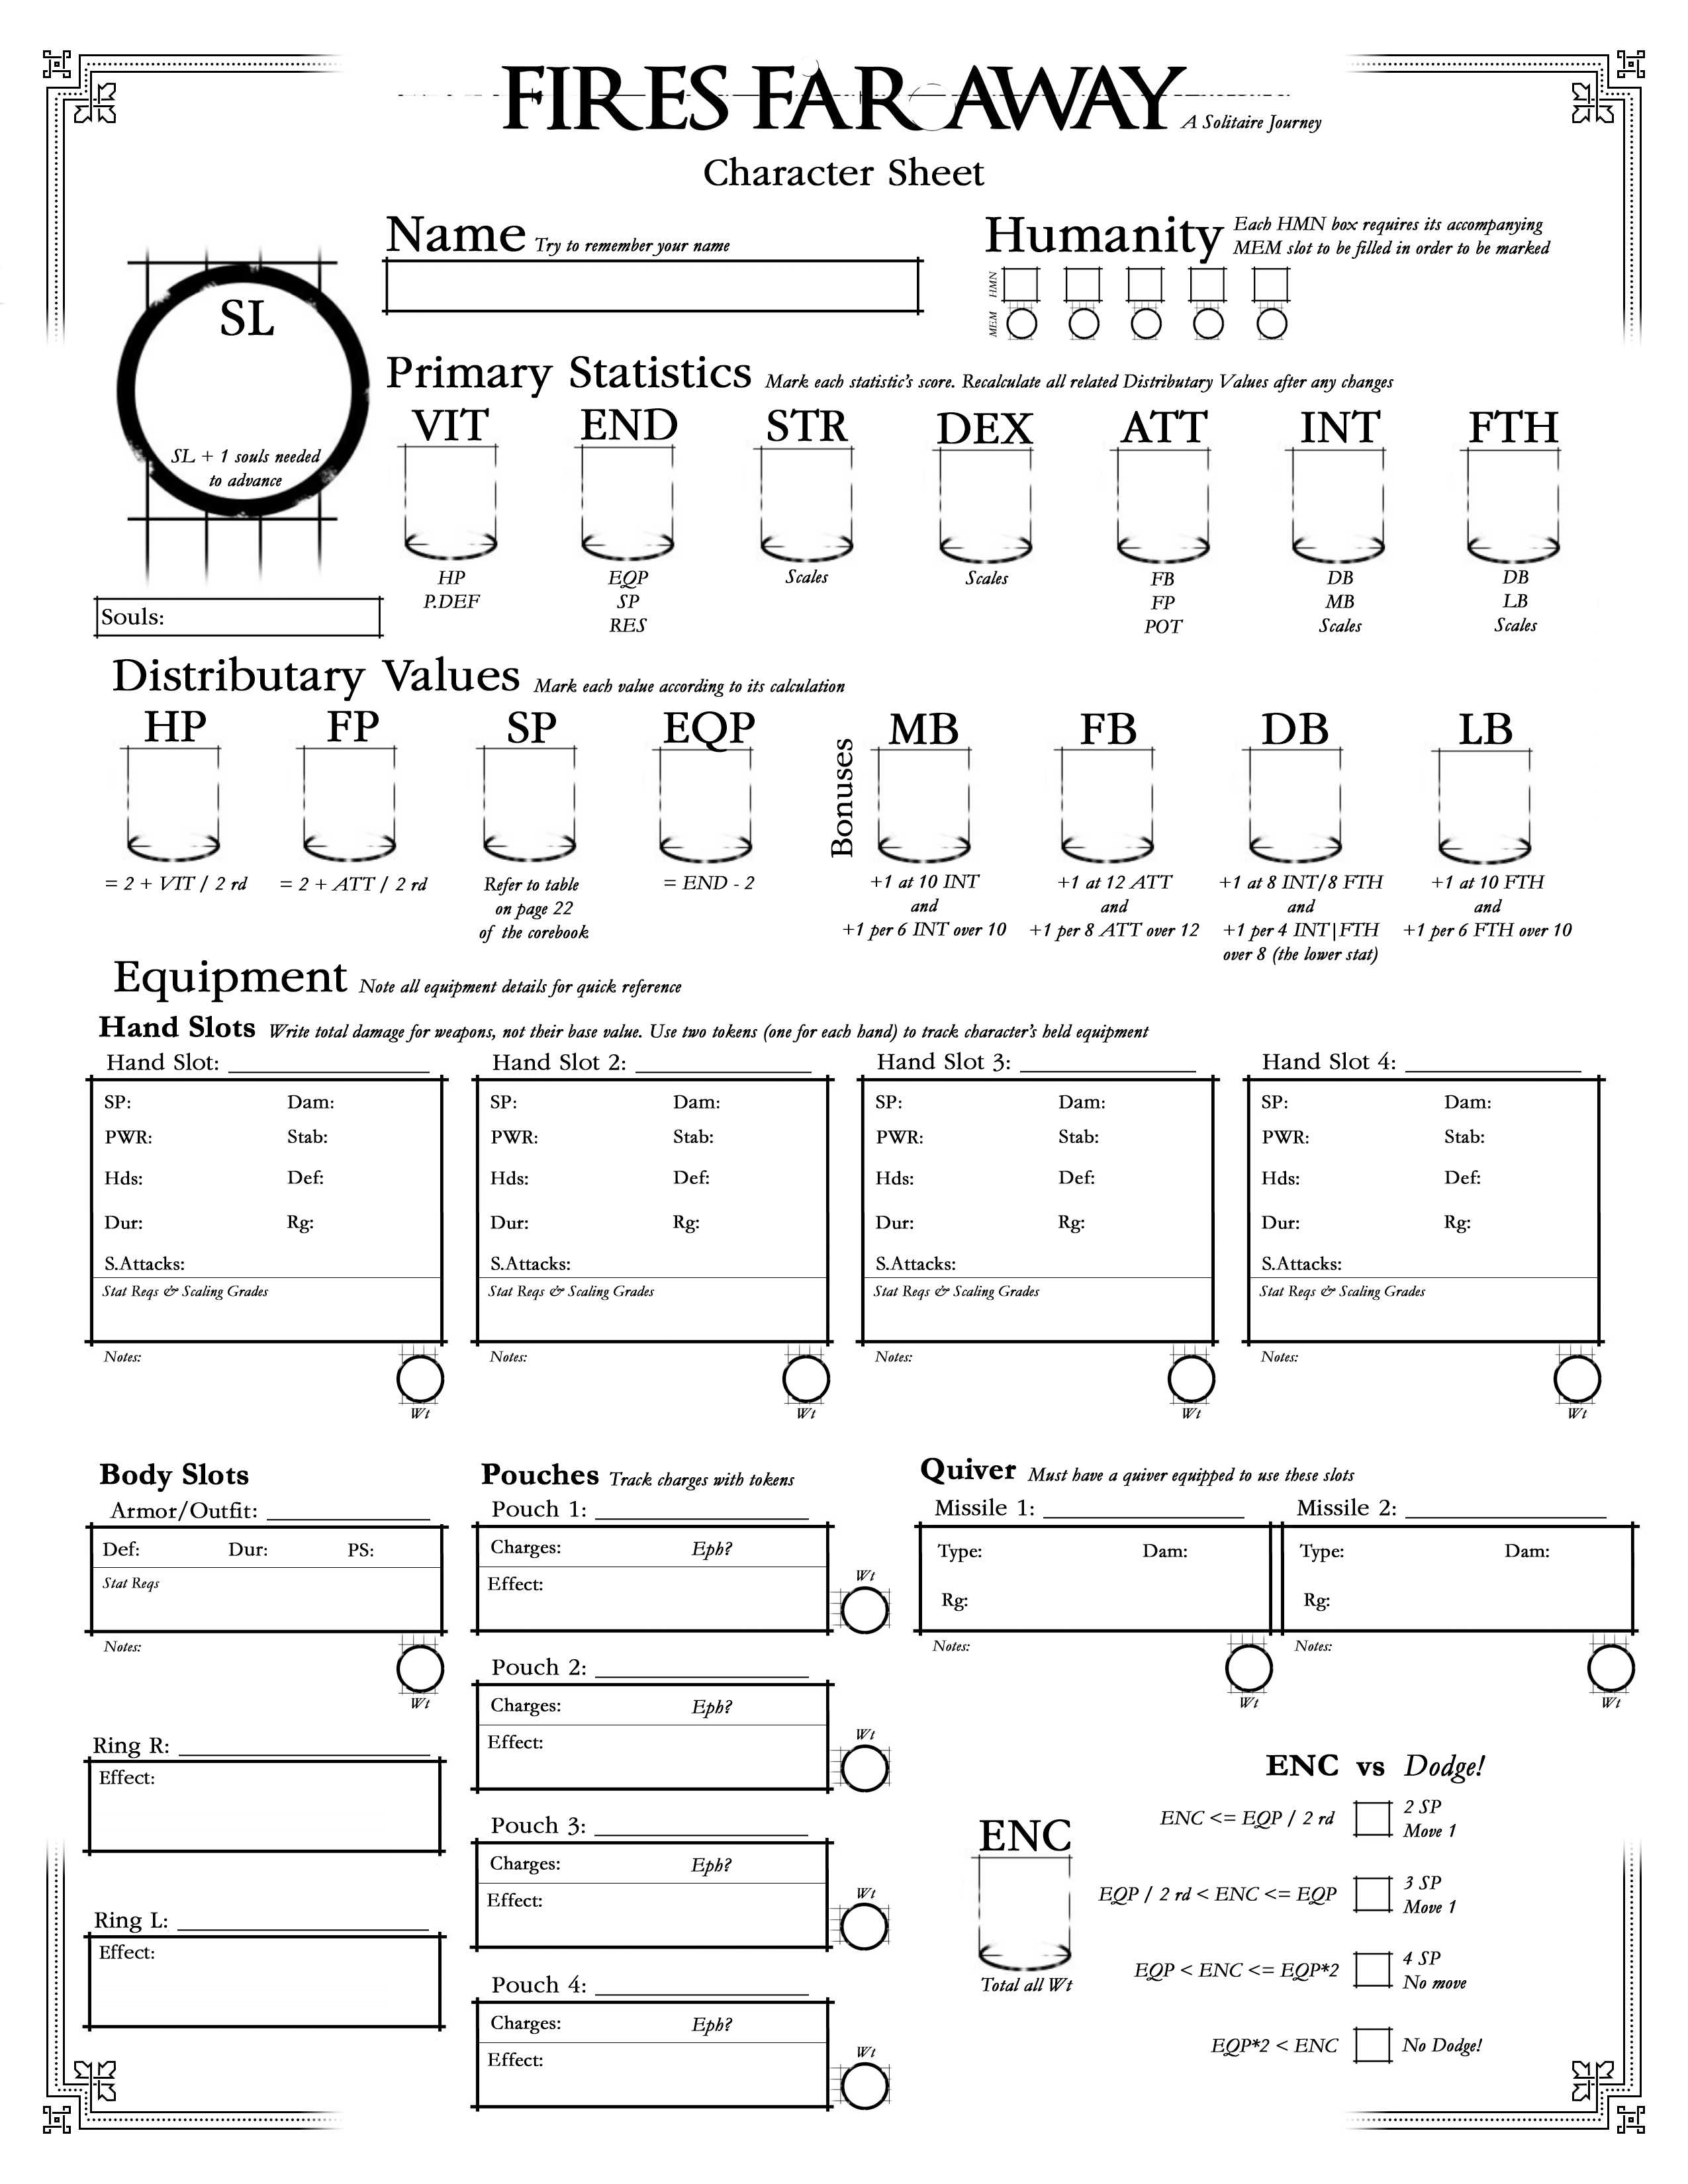
\includegraphics[width=1.22\linewidth]{misc/character_sheet.png}
    }
\end{center}

\end{document}